\section{System Architecture Overview}

The Origin AI architecture is designed as a distributed microservice ecosystem that decouples the UI-heavy frontend from the compute-heavy AI orchestrator. This separation allows for independent scaling, fault isolation, and technology-appropriate implementation (Next.js for the frontend, Python/FastAPI for the backend).

\begin{figure}[!htbp]
    \centering
    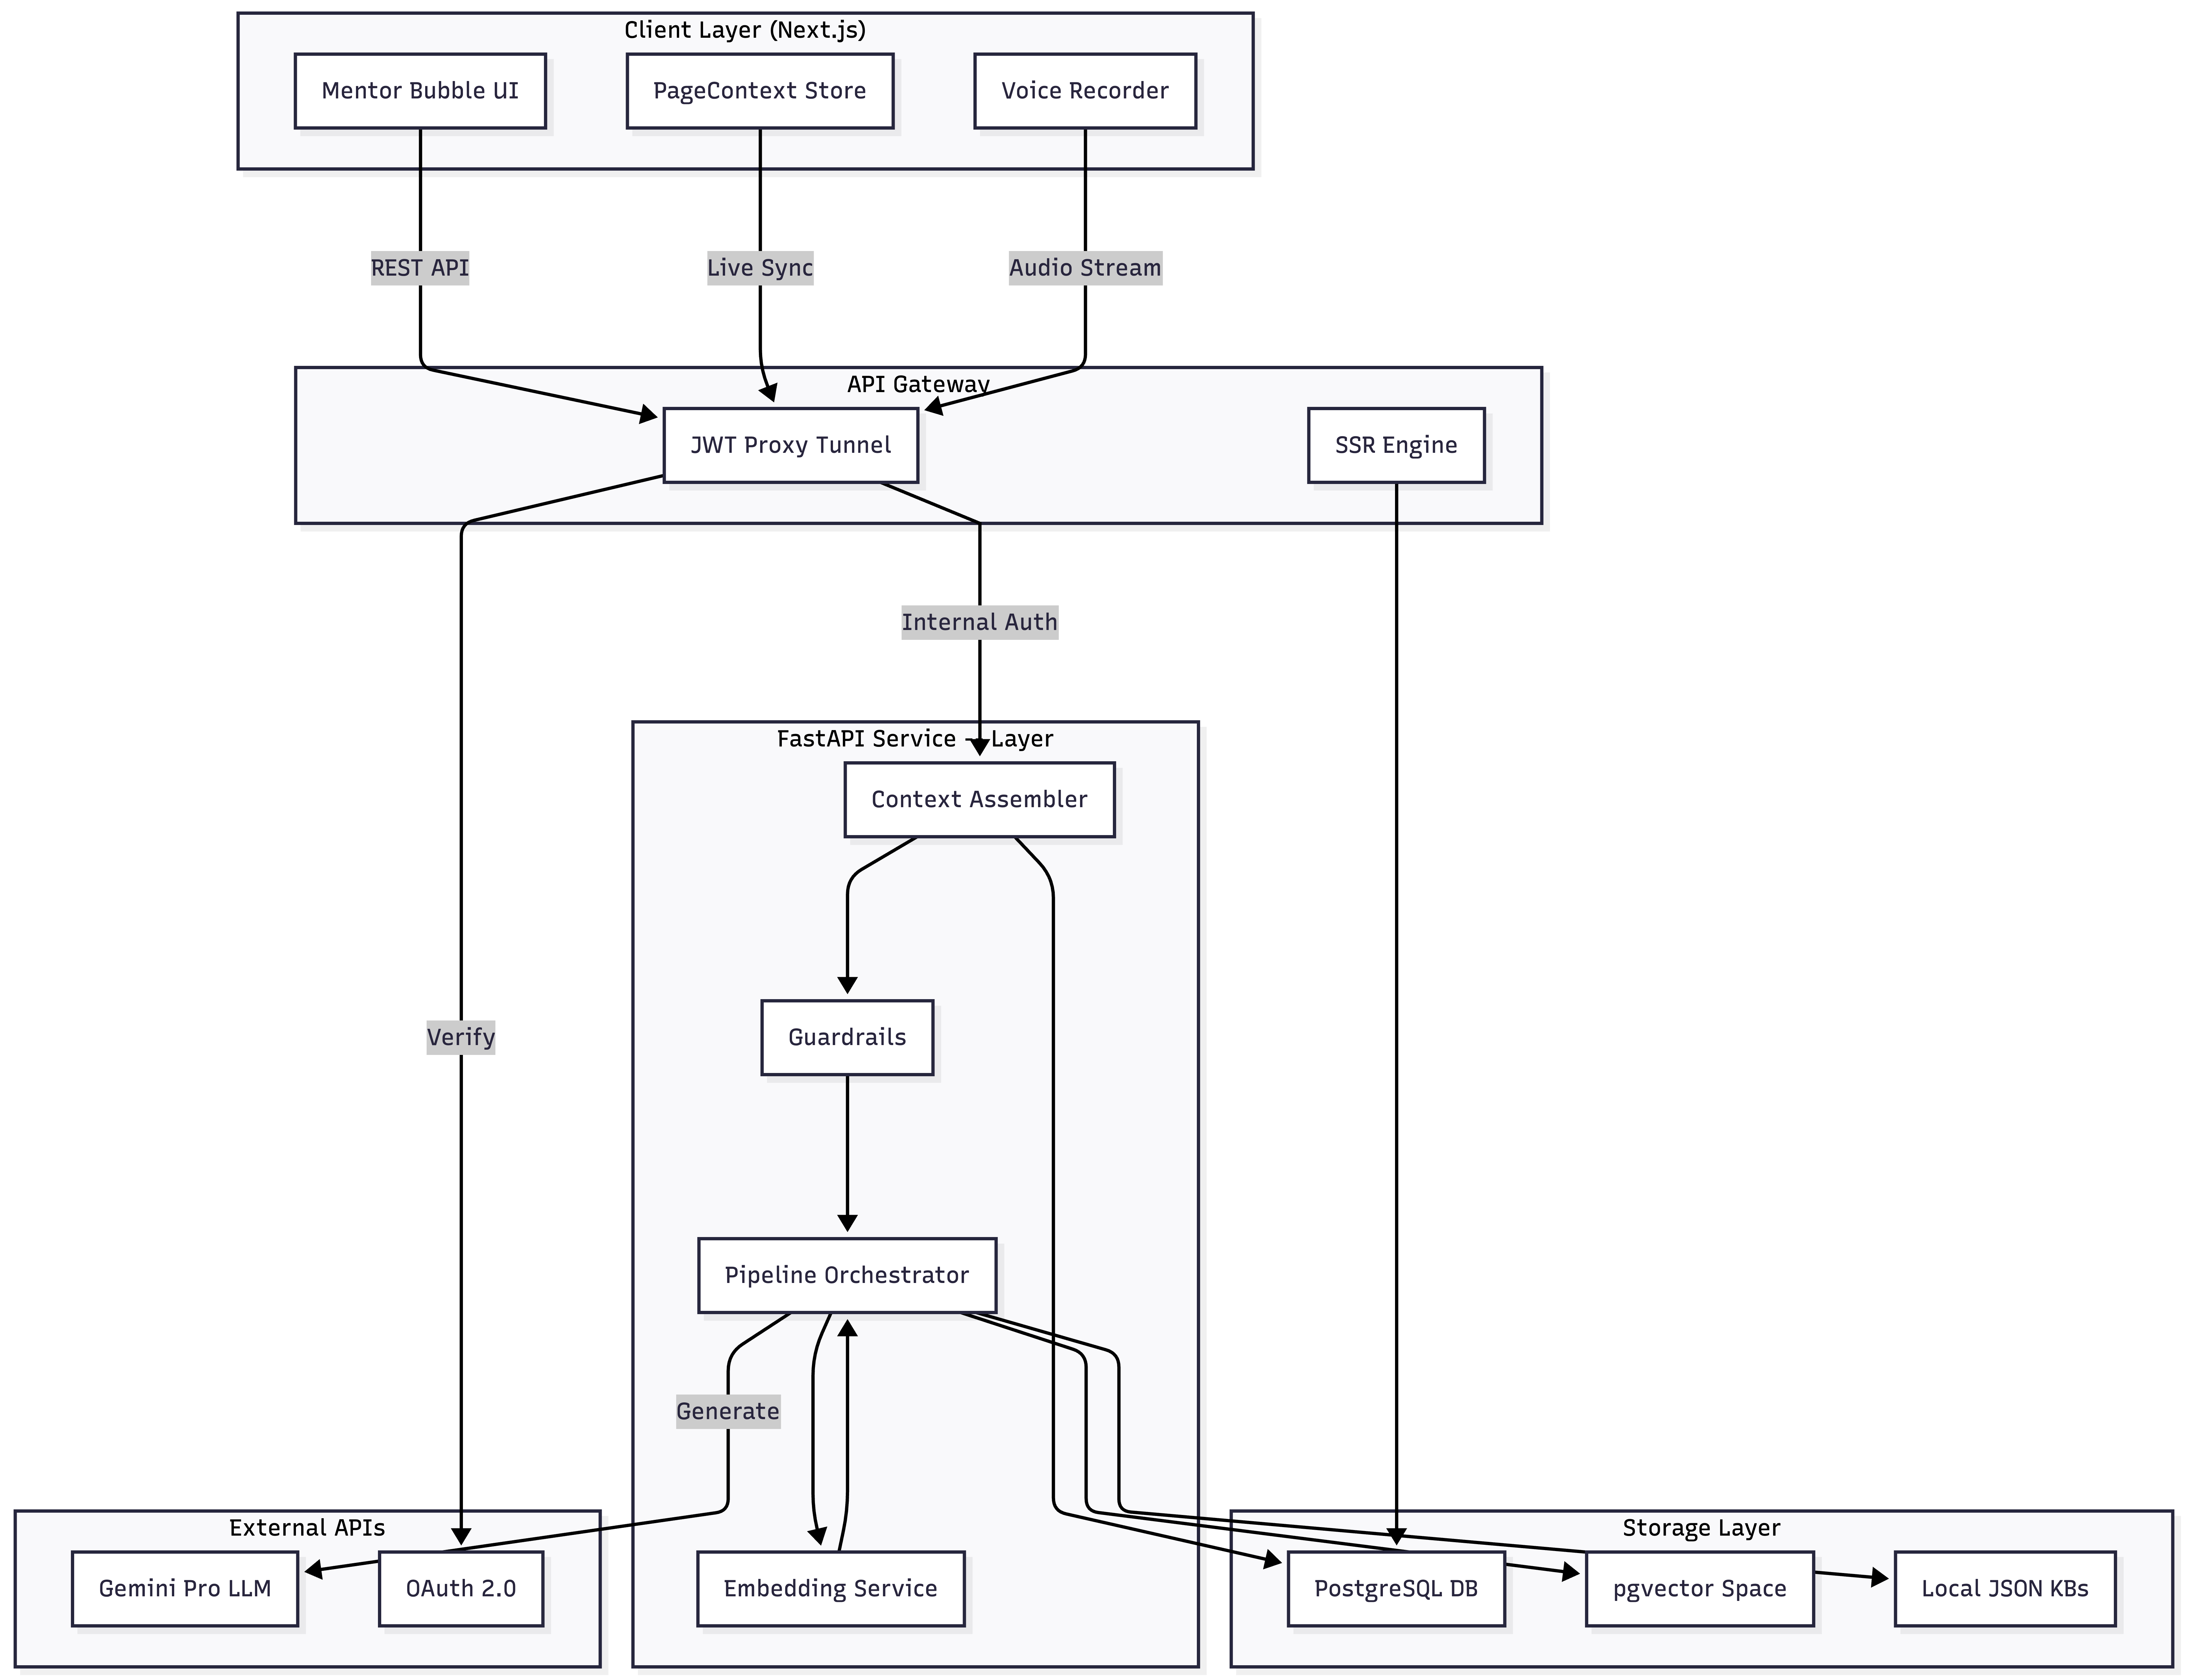
\includegraphics[width=\textwidth,height=0.5\textheight,keepaspectratio]{report_file/architecture.png}
    \caption{Origin AI Technical Architecture}
    \label{fig:technical_architecture}
\end{figure}
\clearpage

The system consists of four main components arranged in a request flow:
\begin{enumerate}
    \item \textbf{Browser (Student UI):} Runs the Next.js application. Contains the floating chat component, highlight capture listener, and page context store.
    \item \textbf{Next.js Application (Vercel):} Serves the frontend assets and provides API routes under \texttt{/api/origin-ai/*}. These routes act as a secure proxy: they validate the student's session cookie, then forward the request to the internal Python microservice with a trusted service token.
    \item \textbf{Python FastAPI Microservice (GCP Cloud Run):} The core AI orchestrator. It receives the request, assembles the 4-layer context, applies guardrails, runs the tiered pipeline, and returns the response.
    \item \textbf{PostgreSQL + pgvector (Neon):} Stores student analytics, mentor sessions, and vector embeddings for semantic retrieval.
\end{enumerate}

\section{The 4-Layer Context Assembly Model}

The fundamental unit of reasoning in Origin AI is the \textbf{OriginAiInput} object. This is a structured data object formed by the fusion of four distinct layers:

\subsection{Layer 1: GlobalContext (Long-Term Memory)}
This layer represents the persistent state of the student, hydrated from the PostgreSQL database.
\begin{itemize}
    \item Weak and Strong topics inferred from performance analytics.
    \item Recent test scores and summaries.
    \item Pinned facts and pending assignments.
\end{itemize}

\subsection{Layer 2: PageContext (Live Environmental State)}
The frontend continuously broadcasts the state of the active screen.
\begin{itemize}
    \item Page kind (test, practice, dashboard).
    \item Active question ID, subject, and chapter.
    \item Solution/hint availability.
\end{itemize}

\subsection{Layer 3: HighlightContext (Granular Selection)}
Captured when a student selects text on the page, enabling the ``Explain this'' flow.
\begin{itemize}
    \item Selected text (up to 500 characters).
    \item Source element metadata.
\end{itemize}

\subsection{Layer 4: UserQuery (Active Intent)}
The final layer is the user's explicit input, which can be text-based or voice-based.

\section{Tiered Orchestration Pipeline}

To achieve cost efficiency, the orchestrator follows a deterministic hierarchy:

\begin{enumerate}
    \item \textbf{Step 1: Stored Solution Lookup:} Immediate K-V lookup for known question IDs.
    \item \textbf{Step 2: Subject-Aware Local Knowledge Base (KB):} Resolution of conceptual doubts using pre-loaded JSON pedagogical atoms.
    \item \textbf{Step 3: BFS Semantic Memory Retrieval:} Semantic search over past session history using pgvector embeddings.
    \item \textbf{Step 4: Synthetic LLM Generation:} Fallback to Large Language Models (Gemini/GPT-4o) with dynamic context injection.
\end{enumerate}

\section{Mathematical Modeling of Cost and Relevance}

Operational cost $C$ for a session with $n$ queries is modeled as:
\begin{equation}
C = \sum_{i=1}^{n} (L_i \cdot P_i)
\end{equation}
Where $L_i \in \{0,1\}$ indicates if an LLM was invoked, and $P_i$ is the price per token.

Context Relevance Score (CRS) is calculated via cosine similarity:
\begin{equation}
CRS(C_p, Q) = \frac{\vec{E}(C_p) \cdot \vec{E}(Q)}{\|\vec{E}(C_p)\| \|\vec{E}(Q)\|}
\end{equation}

\section{Cross-Subject Gating Logic}

To disambiguate multi-disciplinary queries (e.g., ``energy''), we implement a scoring-based gate:
\begin{equation}
score_s = base_s + anchor_s
\end{equation}
The gate requires a confidence floor of $\max(score) \geq 6$ and a margin requirement of $\max(score) - second\_max \geq 3$ to select a subject KB automatically.

\section{Pedagogical Guardrails and Policy Resolution}

The guardrail system implements a state machine that controls the AI's behavior based on the PageContext:

\begin{table}[htbp]
\centering
\caption{Policy Resolution State Machine}
\label{tab:guardrails}
\begin{tabular}{|l|l|l|}
\hline
\textbf{Condition} & \textbf{Policy Mode} & \textbf{AI Behavior} \\ \hline
\texttt{test\_active == true} & \texttt{answer\_blocked} & Block content, provide encouragement. \\ \hline
\texttt{attempted == false} & \texttt{hint\_only} & Socratic nudge, conceptual hint. \\ \hline
\texttt{attempted == true} & \texttt{normal} & Full step-by-step explanation. \\ \hline
\end{tabular}
\end{table}

\section{Request Processing Sequence}

The interaction between the student and the various microservices follows a strictly defined sequence to ensure security and efficiency. The following steps describe the lifecycle of a query:

\begin{enumerate}
    \item \textbf{Trigger:} The student clicks the "Ask Origin AI" button or finishes a voice recording.
    \item \textbf{UI Serialization:} The React frontend serializes the `PageContext` (question ID, subject, mode) and `HighlightContext` (selected text).
    \item \textbf{Secure Handshake:} The Next.js API route validates the student's JWT session. If valid, it appends a secret INTERNAL SERVICE TOKEN and forwards the payload to the Python orchestrator.
    \item \textbf{Orchestration:}
    \begin{itemize}
        \item The Python backend checks the `mode`. If "test", it returns a "Blocked" policy immediately.
        \item It attempts Step 1 (Stored Solution). If found, it returns early.
        \item It attempts Step 2 (Subject KB). If a concept match is found with high confidence, it returns early.
        \item It performs a vector search in Step 3.
        \item Finally, it calls the LLM if needed, injecting the `PageContext` and `GlobalContext` into the system prompt.
    \end{itemize}
    \item \textbf{Response Streaming:} The AI's response is streamed back to the frontend to minimize perceived latency.
\end{enumerate}

\section{Database Schema Design}

The persistence layer is implemented in PostgreSQL \cite{postgresql2024docs} with a comprehensive schema designed to support the entire Origin AI ecosystem. The schema captures user logistics, study tracking, the AI orchestration engine, and the core curriculum.

\begin{itemize}
    \item \textbf{Core Logistics:} The \texttt{origin\_users}, \texttt{origin\_auth\_sessions}, and \texttt{origin\_tasks} tables manage role-based authentication, persistent logins, and user-assigned goals.
    \item \textbf{Study \& Analytics:} The \texttt{origin\_pomodoro\_sessions} and \texttt{origin\_analytics} tables log student focus time and track historical performance, mastery levels, and weak topics.
    \item \textbf{Origin AI Ecosystem:} The \texttt{origin\_ai\_conversations}, \texttt{origin\_ai\_embeddings}, and \texttt{origin\_ai\_knowledge\_base} tables act as the central AI memory. They log multimodal interactions, store pgvector \cite{pgvector2024github} 1536-dimensional semantic embeddings, and maintain pedagogical rules.
    \item \textbf{Curriculum Architecture:} The \texttt{origin\_subjects}, \texttt{origin\_questions}, and 
    \\
    \texttt{origin\_answers} tables form the content repository, allowing teachers to author and map questions to specific syllabi.
\end{itemize}

\subsection{Conceptual Data Model}
The following diagram illustrates the overarching conceptual data model of the Origin AI platform using Object-Oriented Notation, highlighting the primary entities, their attributes, and the behavioral relationships between them.

\clearpage
\begin{figure}[!htbp]
    \centering
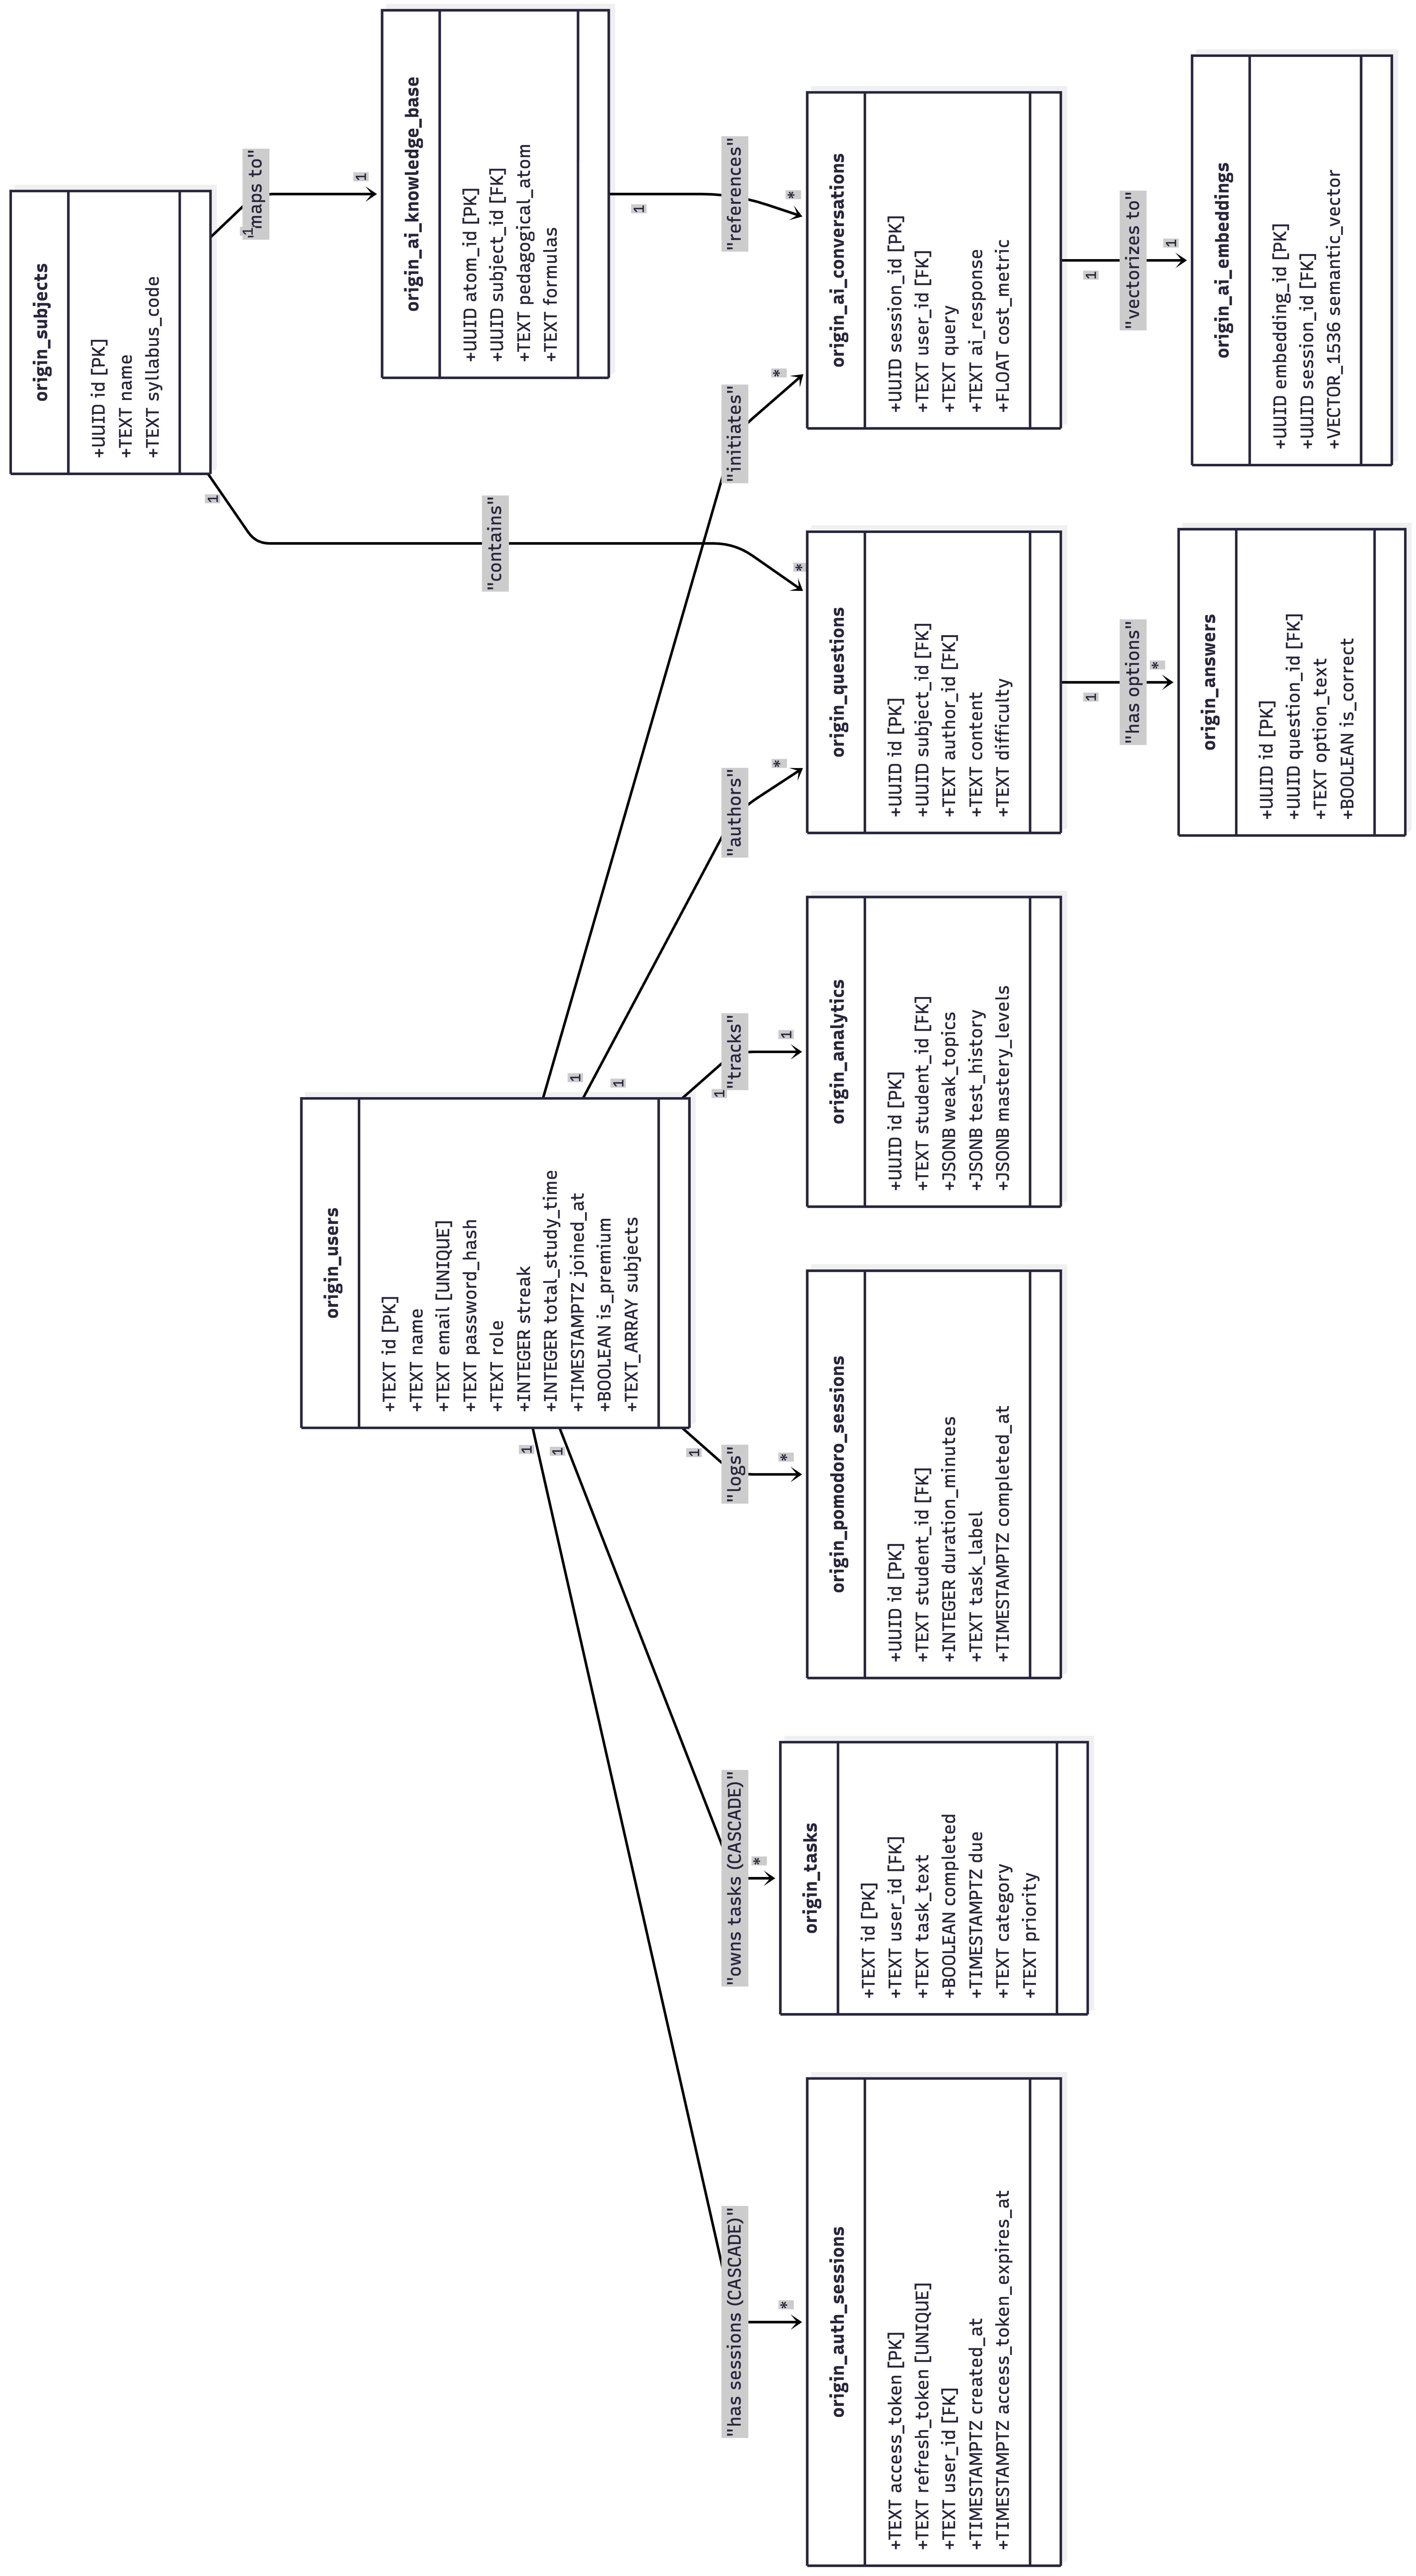
\includegraphics[width=1\textwidth,height=1\textheight]{report_file/db_schema.png}
    \caption{Database Schema Conceptual Model (Object-Oriented Notation)}
    \label{fig:db_schema}
\end{figure}
\clearpage

\subsection{Physical Database Schema}
The following diagram illustrates the exact PostgreSQL physical table layout, defining primary keys, foreign keys, cardinality, and constraints for the backend database architecture.

\begin{figure}[!htbp]
    \centering
    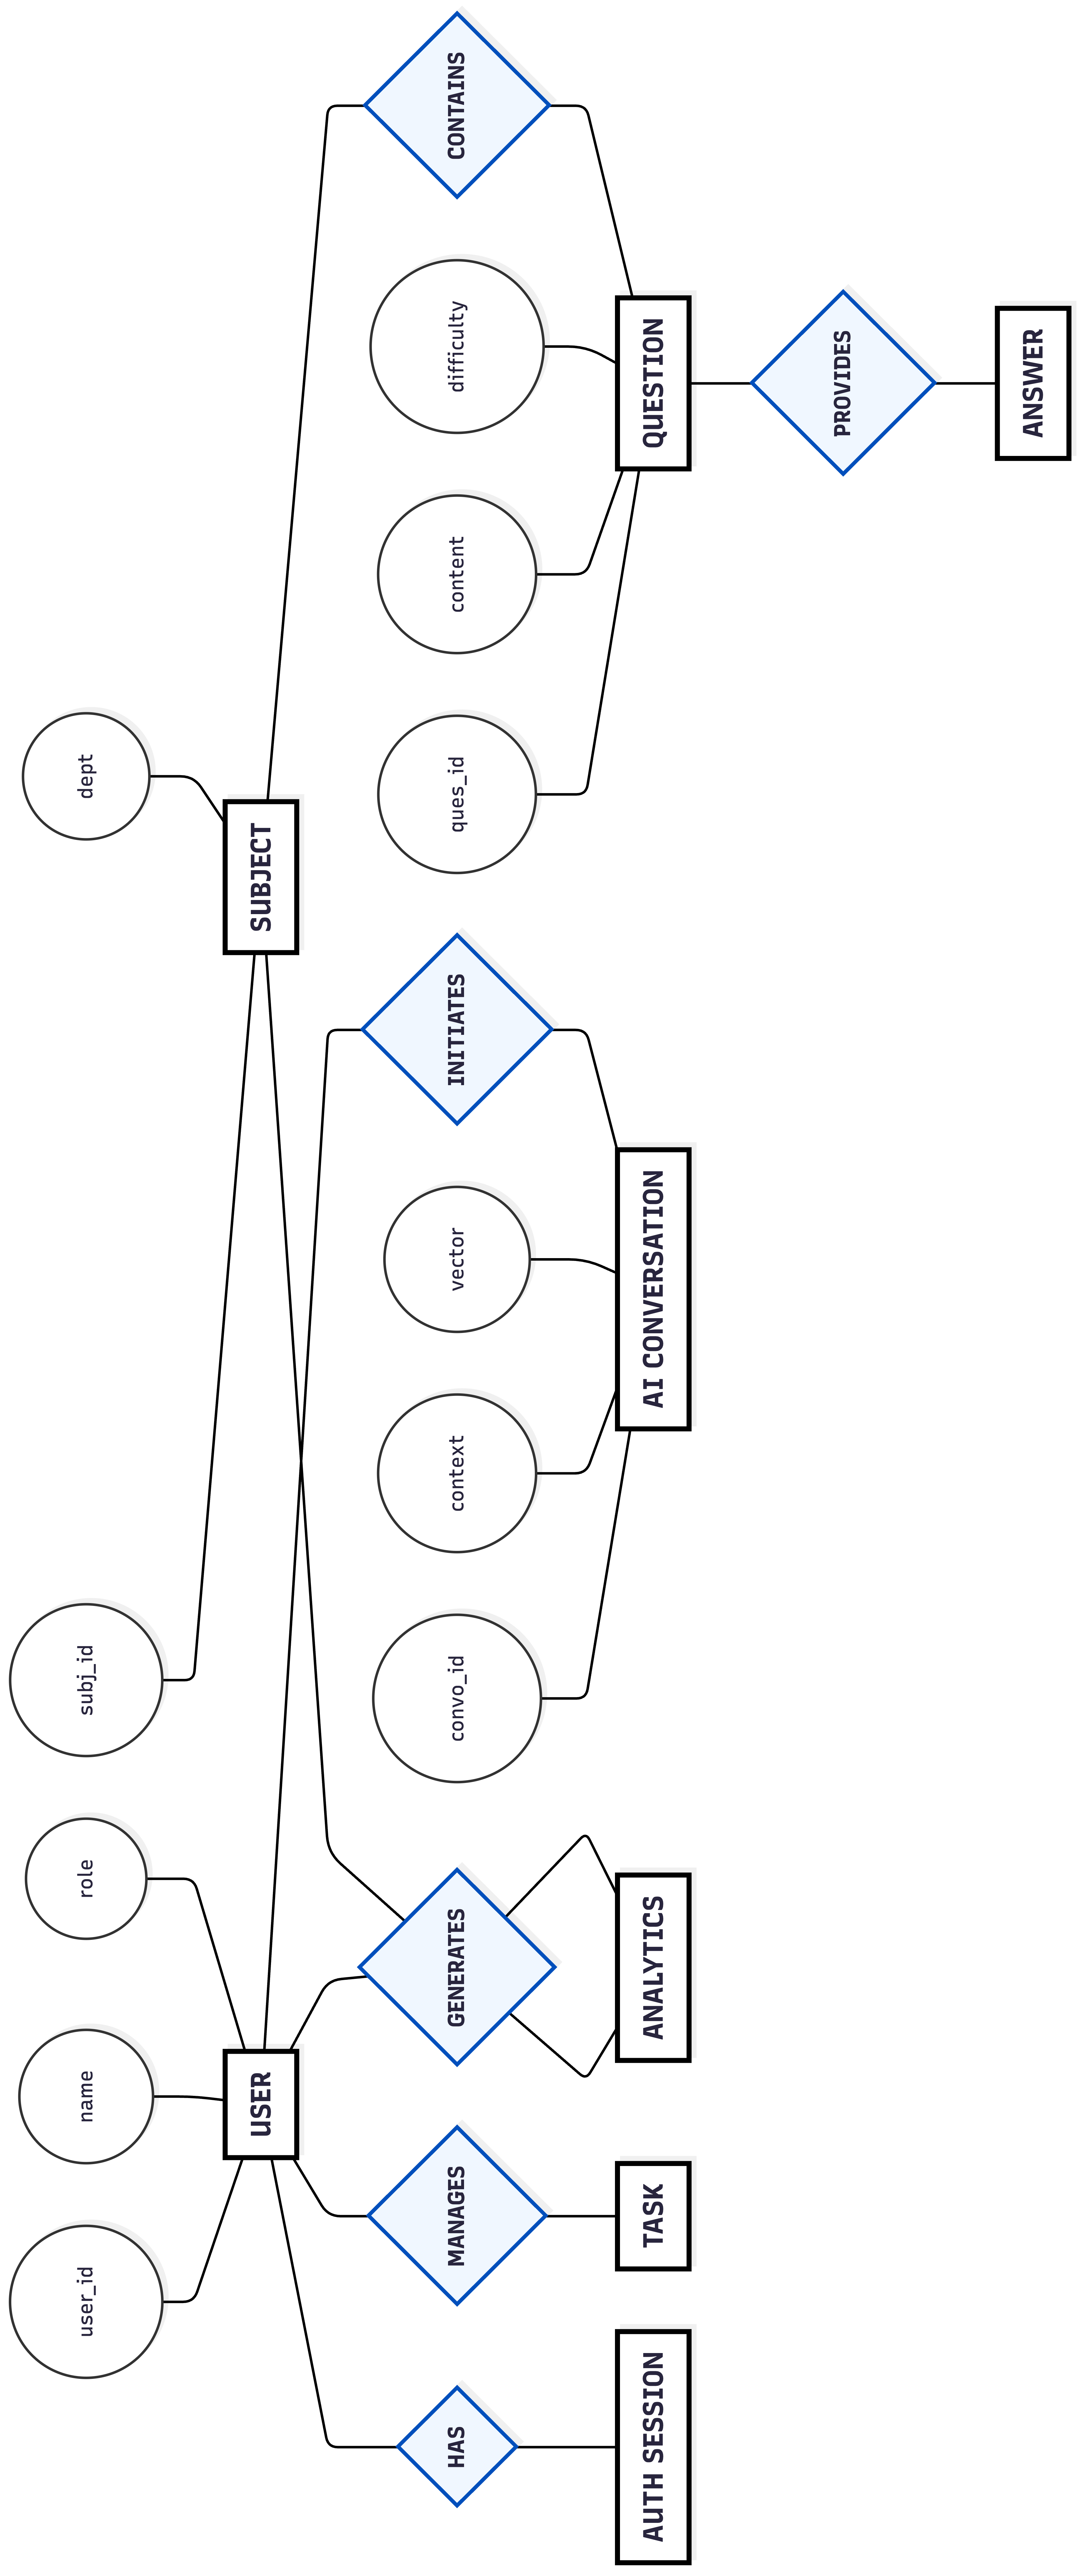
\includegraphics[width=0.7\textwidth,height=0.8\textheight]{report_file/er_diagram.png}
    \caption{Physical Database Implementation Schema}
    \label{fig:er_diagram}
\end{figure}
\clearpage

\section{System Data Flow Analysis}

To fully understand the movement of data across the Origin AI platform, we utilize Data Flow Diagrams (DFDs) which map out the flow of information between external entities, processes, and data stores. 

\subsection{Level 0 Context Diagram}
The Level 0 DFD provides a high-level, bird's-eye view of the system. It illustrates the Origin AI System as a singular processing node and demonstrates how the primary external entities---Students, Teachers, Administrators, and External APIs (like the Gemini LLM)---interact with it. This diagram highlights the core inputs (multimodal queries, telemetric data) and outputs (pedagogical hints, analytics).

\begin{figure}[!htbp]
    \centering
    
\includegraphics[width=0.6\textwidth,height=0.7\textheight]{report_file/dfd_level_0.png}
    \caption{Data Flow Diagram - Level 0 (Context Diagram)}
    \label{fig:dfd_level_0}
\end{figure}
\clearpage

\subsection{Level 1 Process Decomposition}
The Level 1 DFD decomposes the singular system node into five core sub-processes: Client State \& UI, Auth \& Session Routing, Context Assembler, Tiered Orchestrator, and Semantic Memory Engine. It also maps the interactions with internal datastores such as PostgreSQL for analytics and pgvector for the Knowledge Tree. This diagram maps the exact lifecycle of a student's query from the UI down to the database and external LLM layer.

\begin{figure}[!htbp]
    \centering
    
\includegraphics[width=0.8\textwidth,height=0.73\textheight,keepaspectratio]{report_file/dfd_level_1.png}
    \caption{Data Flow Diagram - Level 1 (Process Decomposition)}
    \label{fig:dfd_level_1}
\end{figure}
\clearpage

\section{Role-Based Access Flow}
Origin AI caters to multiple user personas. The following diagram illustrates the distinct user journeys based on role authentication. For students, the flow splits into practice mode (allowing hints) and test mode (where assistance is blocked by guardrails). For teachers, the flow is focused on analytics aggregation and identifying class-wide weak topics. For administrators, the flow emphasizes cost monitoring and database management.

\begin{figure}[!htbp]
    \centering
    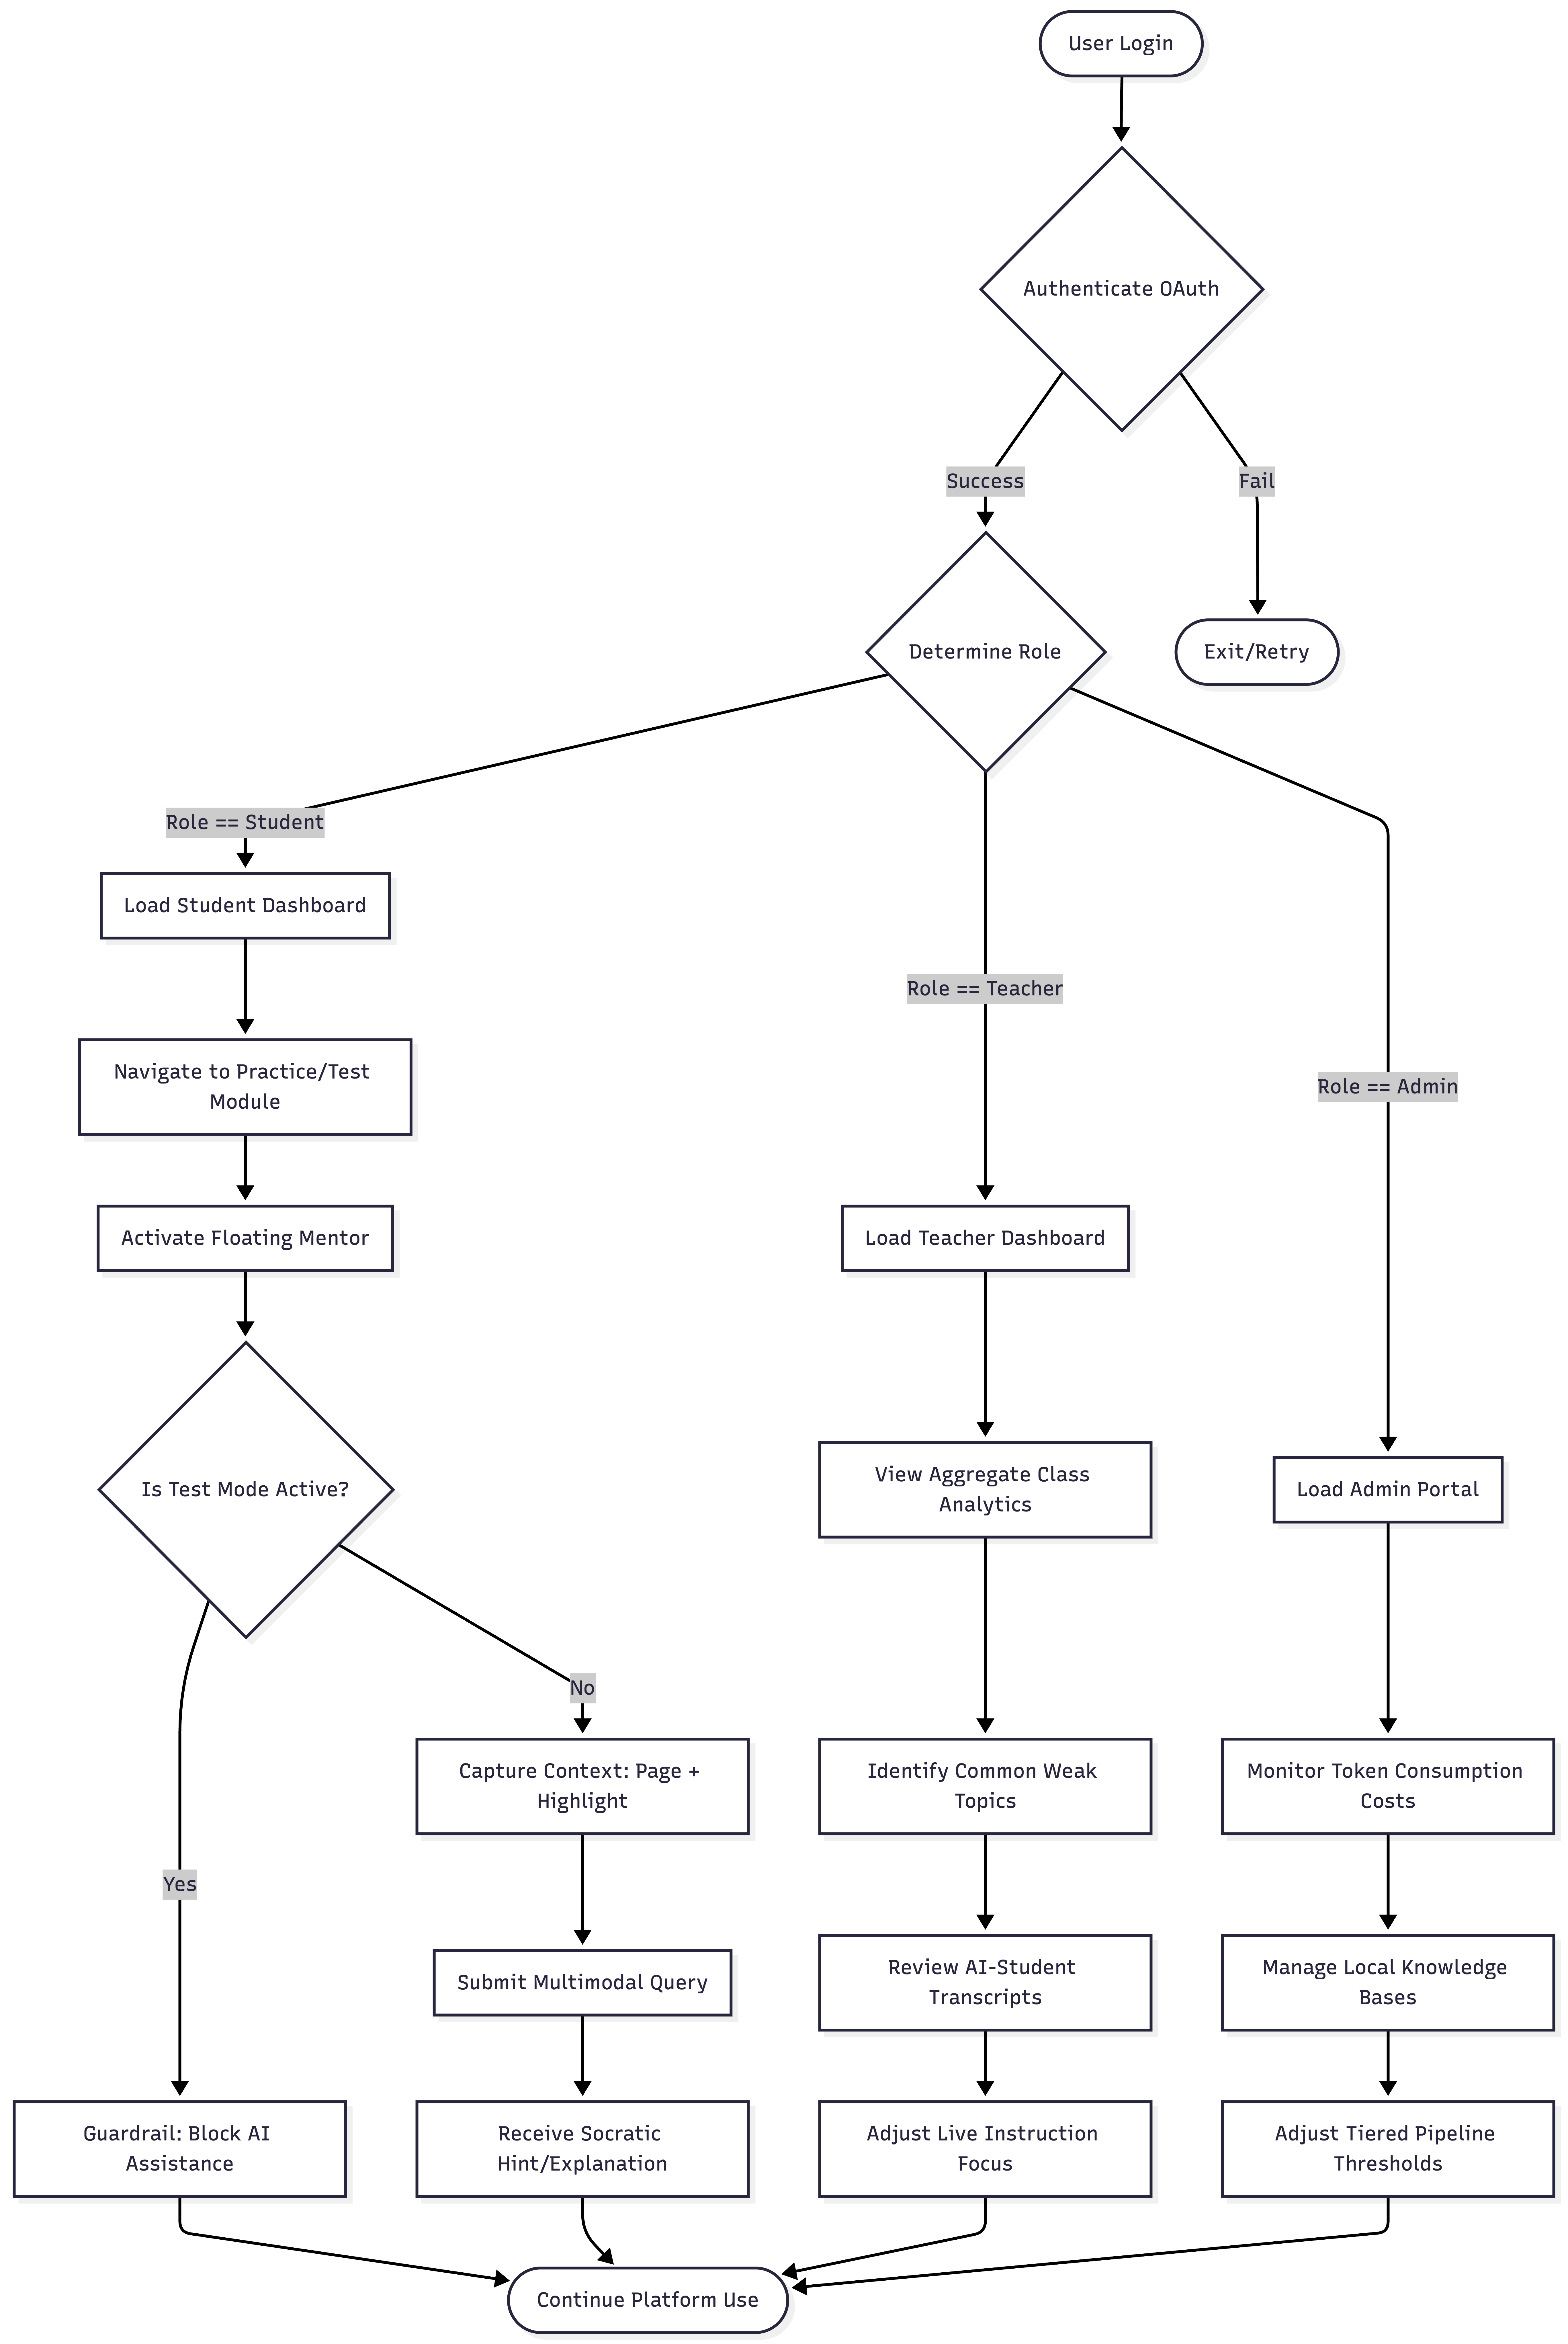
\includegraphics[width=\textwidth,height=0.75\textheight,keepaspectratio]{report_file/role_flow.png}
    \caption{Role-Based Access and Data Flow}
    \label{fig:role_flow}
\end{figure}
\clearpage

